\section{\administrationgroup{}}
\label{sec:productsubsystem}
%\section{Sub-System}
In this section the \subsystem{} implemented by our group is evaluated. 
This section is divided into the different aspects of this \subsystem{}.
The focus is on both design and implementation choices.
%The subsystem created can be split into two parts, the management part and the project group room and are implemented differently.

\subsection{Project Group Structure}
We decided to implement the concept of project groups in Moodle to satisfy the system definition of \system{}.
We did not make a distinction between projects and groups but combined the two into one entity, which made the system more simple. 
If the distinction should be made the concept of projects can be added to the system and a link between project groups and projects must be created.
A project would encapsulate the over-arching theme of a semester, e.g.\ Application Development in our case.
The project groups would be the instantiations, so to speak, of the project -- MyMoodle in our case.
% based on the appropriate quantity relation. 
%A project is as described in section XXX\todo{ref -- to what?} an entity which is per semester based and can contain several groups. %what is the meaning of this?
A project can have a page in the same way a project group has a page, which will allow for collaboration and communication between groups in a semester. 

An alternative approach to consider is to make project groups nestable; that is to allow a project group to have a parent.
This would give even further flexibility.
This will allow for large groups of students to be split into several subgroups, which would make a student part of his subgroup and its parent group.
It can be implemented using a recursive tree structure.
Consider our case, we are four people work in a \subgroup{}, this \subgroup{} along with three other constitute the group developing \system{}.
The \system{} group is part of a semester project with the theme Application Development, that has another group as well -- the Android group.
In our system this can be accomplished by making a project group for both \subgroup{}s, groups, and the semester.
A student is then part of the appropriate project groups.
The difference between a recursive tree structure and our implementation is illustrated in \figref{fig:groupstructure}.


\begin{figure}%
        \begin{subfigure}[b]{0.45\textwidth}
                \centering
                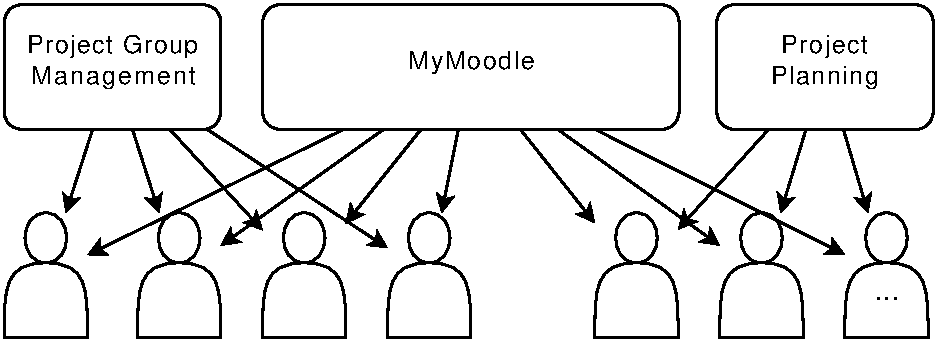
\includegraphics[width=\textwidth]{images/FlatGroupStructure.pdf}
                \morscaption{Flat group structure}
                \label{fig:groupstructure:flat}
        \end{subfigure}%
				\quad
        \begin{subfigure}[b]{0.45\textwidth}
                \centering
                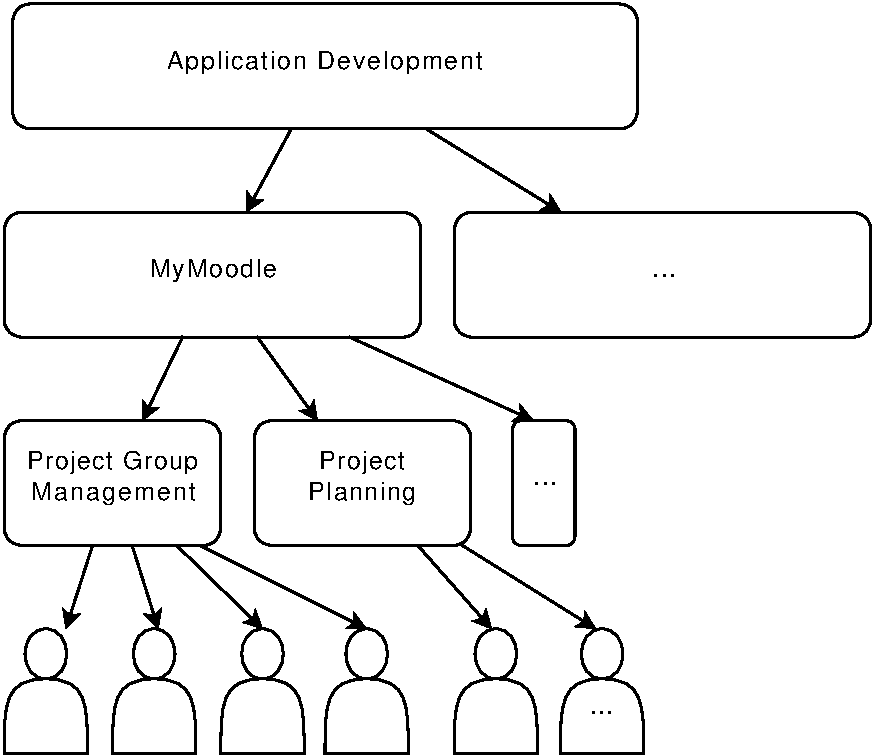
\includegraphics[width=\textwidth]{images/RecursiveTreeStructure.pdf}
                \morscaption{Recuresive tree group structure}
                \label{fig:groupstructure:rec}
        \end{subfigure}%
\morscaption{Recursive tree structure and our our flat structure}%
\label{fig:groupstructure}%
\end{figure}



\subsection{Virtual Group Room}
%% Team vs. Shared
In \secref{sec:virtualMeetingPlace} we decide to implement the virtual group room to satisfy the need for a virtual meeting place.
Each project group has its own room for collaboration. 
%The shared room is infeasible, as argued in that section. 

The virtual group room is implemented as a container for blocks, which made the inter-group integration less time consuming by having a common interface between the virtual group room and the \detdeandrelaver{}s.
%specifying how the different groups could add their work to the project group room. 
At the same time it gives a great flexibility since the individual group can organize the blocks themselves and add arbitrary blocks.

%%% Context
In the implementation of the virtual group room we created our own context, which gives a better solution compared to linking project groups to courses. 
Such a link would create an unnatural relation, which does not reflect the problem domain.  

\subsection{User Interface}
In the last demo meeting with Lene W. Even (seen in \appref{sec:lenedemoone}) she expressed some dissatisfaction with how the filtering functionality of the project groups work.
It would be easier for some users to use the filtering of project groups as a search query instead.
Specifically this means that filters should as default be discarded when adding a new filter.
It should still, however, be possible to have more than one filter.

Additionally, it should be possible to filter the project groups on more attributes.
It should be possible to filter project groups by attributes of the members of the project group.
These attributes could be the year the students started their education, their group room (if they have one), their email, and the city in which they study.

%Kun skrevet om 

\subsection{Administration}
\label{sec:evalAdministration}
We decided that management of project groups should only be done by administrative personnel. 
This is not a final decision and we reckon that allowing users to create their own project groups is not necessarily a bad idea. 
With student management of project groups there are several constraints, which must be considered; these are discussed in \secref{sub:studentmangement}. 
The constraints that should be considered are mainly security and integrity related.
Examples of constraints that must be considered include users cannot delete project groups prematurely.
Many of the constraints that apply to student management also apply to \admpers{} management, but we believe that \admpers{} are less likely to perform any destructive action than students.
First of all it is possible for \admpers{} to receive training in the usage of the system, such training is much more expensive to give to students because there is simply more students than \admpers{}\todo{Er det overhoved rigtigt?}.
Secondly it is the job of the \admpers{} to administrate entities in the university, hence they have a responsibility that students do not.
%The resulting system and its usage thereof will be slightly different.

When the \admpers{} manages project groups the system has a possibility to become authoritative.
That is, the system can be used as primary project group database. 
To become an authoritative project group database the structure of the project groups and projects, which are discussed in \secref{sub:divProjGroup}, must be changed to be more general to support all structures at the university (see \appref{sec:mikael}) and the number of Moodle installations at AAU must be reduced to one. \todo{why not a hundred?}
With student management the authority of the system is removed and will only be a tool for students and their supervisors.




\subsection{Testing}
% Testing
In the process of creating our \subsystem{} of \system{} we used TDD.
It worked well for us during the implementation of the core functionality, because it made any misconceptions we had of the Moodle core functions clear.
We did not use TDD for the creation of user interfaces.

Testing of the developed system is done using the SimpleTest framework. 
A framework already included in Moodle and hence we did not have to spend time integrating a testing framework.

The result of the tests showed a good code coverage percentage and a large amount of test cases which combined with the demo meetings shows that the \subsystem{} is stable. 
The system does not have a high criticality and attempting to achieve a more thoroughly test suite is not necessary. 
%A worst-case scenario is that a bug in \system{} causes data loss. 

In the worst-case, e.g.\ the system is unavailable and all data is lost, the users does not lose money or lives, assuming that \system{} is not used as an authoritative system.
Hopefully this will never occur, but cannot be ruled out since it is impossible to declare a program bug free using testing.
To overcome this potential loss the database and user files must be backed up.
